% Chapter 02
\chapter{A comparison of gene expression and DNA methylation 
patterns across tissues and species}\label{ch:tb}
\section[Abstract]{Abstract\footnotemark}

Previously published comparative functional genomic data sets from primates using frozen tissue samples, including many data sets from our own group, were often collected and analyzed using non-optimal study designs and analysis approaches. In addition, when samples from multiple tissues were studied in a comparative framework, individual and tissue were confounded. We designed a multi-tissue comparative study of gene expression and DNA methylation in primates that minimizes confounding effects, by using a balanced design with respect to species, tissues, and individuals. We also developed a comparative analysis pipeline that minimizes biases due to sequence divergence. Thus, we present the most comprehensive catalog of similarities and differences in gene expression and methylation levels between livers, kidneys, hearts, and lungs, in humans, chimpanzees, and rhesus macaques. We estimate that overall, only between 7 to 11\% (depending on the tissue) of inter-species differences in gene expression levels can be accounted for by corresponding differences in promoter DNA methylation. However, gene expression divergence in conserved tissue-specific genes can be explained by corresponding inter-species methylation changes more often. Finally, we show that genes whose tissue-specific regulatory patterns are consistent with the action of natural selection are highly connected in both gene regulatory and protein-protein interaction networks.  

\footnotetext{Citation for chapter: Blake LE*, Roux J*, Hernando-Herraez I, Banovich NE, Garcia-Perez R, Hsiao CJ, Eres I, Chavarria C, Marques-Bonet T, Gilad Y. A comparison of gene expression and DNA methylation patterns across tissues and species. bioRxiv.  doi: https://doi.org/10.1101/487413. * denotes equal contribution.}

\section{Introduction}\label{ch02-introduction}

Gene regulatory differences between humans and other primates are hypothesized to underlie human-specific traits \cite{RN1343}. Over the past decade, dozens of comparative genomic studies focused on characterizing mRNA expression level differences between primates in a large number of tissues (e.g., \cite{RN3251, RN2106, RN1, RN1931, RN3250}), typically focusing on differences between humans and other primates. A few studies have also characterized inter-primate differences in regulatory mechanisms and phenotypes other than gene expression levels, such as DNA methylation levels, chromatin modifications and accessibility, and protein expression levels \cite{RN3285, RN2110, RN2111, RN2113, RN2091, RN3288, RN3287, RN3286, RN3284}. These studies often construct catalogs of gene expression levels and other mechanisms. These catalogs have been useful to better understand the evolutionary processes that led to adaptations in humans \cite{RN3426, RN1339, RN2106, RN3419, RN1800, RN1931, RN3425, RN3422, RN3250, RN3421, RN3435, RN3424, RN1798, RN2091, RN3427} and ancestral or derived phenotypes that may be relevant to human diseases \cite{RN2055, RN1342}. 
One caveat that is shared among practically all comparative studies in primates is related to difficulty in obtaining multiple tissue samples from the same individual. To date, there have been no published comparative studies in primates that have analyzed multiple tissues sampled from the same individuals across multiple species in a balanced design \cite{RN1342}. As a result, regulatory differences between tissues are always confounded with regulatory differences between individuals \cite{RN2106, RN1, RN4091, RN2091}. In turn, catalogs from these studies can not be used to compare tissue-specific regulatory differences between species to inter-tissue differences in regulatory variation within species (see Discussion in \cite{RN2091}).
Our group and others often use previously published catalogs of comparative data in primates in our different studies. While we do not expect previously observed patterns to be erroneous, we are aware that data on gene-specific inter-species regulatory differences, and especially data that pertain to comparisons of divergence across tissues, may be inaccurate for the reasons we discussed above. We thus designed the current study to produce a new comprehensive catalog of comparative gene expression and DNA methylation data from humans, chimpanzees, and rhesus macaques, attempting to minimize possible confounders. 
The goal of our study is not to challenge previous conclusions or document specific differences between the current and previous data. Instead, we aim to provide a new and more accurate comparative catalog of inter-tissue and inter-species differences in gene regulation between humans and other primates, with substantial sample and study design documentation. Overall, we believe that this catalog can be useful for many future applications and can serve as a new benchmark for regulatory divergence in primates. 

\section{Results}\label{ch02-results}

\subsection{Study design and data collection 
}\label{bacterial-infection-induces-large-changes-in-gene-expression}

To comparatively study gene expression levels and DNA methylation patterns in primates, we collected primary heart, kidney, liver and lung tissue samples from four human, four chimpanzee, and four rhesus macaque individuals (Figure 1A, Supplemental Table S1A). From these 48 samples, we harvested RNA and DNA in parallel (Methods). After confirming that the RNA from all samples was of acceptable quality (Supplemental Table S1B; Supplemental Fig. S1A), we performed RNA-sequencing to obtain estimates of gene expression levels. Additional details about the donors, tissue samples, sample processing, and sequencing information can be found in the Methods and Supplemental Table S1.
We estimated gene expression levels using an approach designed to prevent biases driven by sequence divergence across the species (similar to the approach of \cite{RN4207}). Briefly, we first mapped RNA-sequencing reads to each species' respective genome, and to compare gene expression levels across species, we only calculated the number of reads mapping to exons that can be classified as clear orthologs across all three species (Supplemental Table S1B). We excluded data from genes that were lowly expressed in over half of the samples as well as data from one human heart sample that was an obvious outlier, probably due to a sample swap (Supplemental Fig. S2A-B). We normalized the distribution of gene expression levels to remove systematic expression differences between species (maximizing the number of genes with invariant expression levels across species corresponds to our null hypothesis; see Methods). Through this process, we obtained TMM- and cyclic loess-normalized log2 counts per million (CPM) values for 12,184 orthologous genes to be used in downstream analyses (Supplemental Table S2).
Elements of study design, including sample processing, have previously been shown to impact gene expression data (Gilad and Mizrahi-Main 2015). Consequently, we tested the relationship between a large number of technical factors recorded throughout our experiments and the biological variables of interest in our study, namely tissue and species (Methods, Supplemental Materials, Supplemental Table S3A-B). We found that there were no technical confounders with tissue but two technical factors were confounded with species: time postmortem until collection and RNA extraction date (Supplemental Fig. 1B-1C). Due to the opportunistic nature of sample collection, these confounders are practically impossible to avoid in comparative studies in primates (especially apes). We discuss possible implications of these confounders throughout the paper.  

\subsection{Gene expression varies more across tissues than across species
}\label{joint-analysis-identifies-bacteria-specific-response-genes}

We first examined broad patterns in the gene expression data. A principal component analysis (PCA) indicated that, as expected \cite{RN3278, RN1, RN3279}, the primary sources of gene expression variation are tissue (Figure 1B, regression of PC1 by tissue = 0.81; P < 10-14; regression of PC2 by tissue = 0.70; P < 10-10; Supplemental Tables S1A-B and S3A-B), followed by species (regression of PC2 by species = 0.27; P < 10-3; Supplemental Tables S1A-B and S3A-B). This pattern is also supported by a clustering analysis based on the correlation matrix of pairwise gene expression estimates across samples (Supplemental Fig. S3). We then confirmed that, globally, gene expression levels across tissues from the same individual are more highly correlated than gene expression levels across tissues from different individuals (Supplemental Fig. S2C). This observation supports the intuitive notion that collecting and analyzing multiple tissues from the same individual is highly desirable in functional genomics studies. 
We sought further explicit evidence that a study design incorporated balanced collection of multiple tissues from the same individuals is more effective. To do so, we used data from the GTEx Consortium (The GTEx Consortium 2017) for lung and heart. We first identified differentially expressed (DE) genes between lung and heart using all of the available GTEx data; we designated these classifications, which are based on hundreds of samples, as the ``truth'' (Supplemental Materials; Supplemental Table S3E). Next, we repeatedly identified DE genes between lung and heart using GTEx data from randomly chosen sets of just 4 samples from each tissue, and compared the results to DE genes identified from an equivalent analysis of sets of 4 samples from each tissue, in which the tissue samples originated from the same donor. Compared to the ``true classification'' based on the entire GTEx dataset, DE analyses using data from samples of tissues that are matched for donors result in a higher ratio of true positives to false positives than analyses using samples from tissues that are unmatched for donors (P = 0.03; Supplemental Table S3F). Given the small number of false positives in both datasets, study design is unlikely to impact large-scale, highly robust trends across species. However, this study design choice is particularly important if one is interested in individual genes (as demonstrated by an example in Figure 1C). 

\subsection{Putatively functional tissue-specific gene expression patterns 
}\label{infection-induced-response-eqtls-are-shared-across-bacterial-infections}

To analyze the pairwise regulatory differences across tissues and species, we used the framework of a linear model (see Methods). We first identified (at FDR = 1\%) 3,695 to 7,027 (depending on the comparison we considered) differences in gene expression levels between tissues, within each species (Table 1; Supplemental Table S4). Overall, the patterns of inter-tissue differences in gene expression levels are similar in the three species, significantly more so than expected by chance alone (P < 10-16, hypergeometric distribution; Supplemental Materials; Supplemental Table S5). A range of 17 to 26\% of inter-tissue DE genes have conserved inter-tissue expression patterns in all three species (Supplemental Table S5). Regardless of species, we found the fewest inter-tissue DE genes when we considered the contrast between liver and kidney, and the largest number of DE genes between liver and either heart or lung (Table 1; Supplemental Table S4B). Unfortunately, since our data were produced from bulk RNA-sequencing, we were unable to determine the impact of cell composition on the number of inter-tissue DE genes. 
We used the same framework of linear modeling to identify gene expression differences between species, within each tissue (Supplemental Table S4A). Depending on the tissue and species we considered, we identified between 805 to 4,098 inter-species DE genes (at FDR = 1\%; Table 1, Supplemental Table S4C). As expected given the known phylogeny of the three species, within each tissue, we classified far fewer DE genes between humans and chimpanzees than between either of these species and rhesus macaques (Supplemental Table S4B). 
It is a common notion that genes with tissue-specific expression patterns may underlie tissue-specific functions. Previous catalogs of such patterns in primates were always confounded by the effect of individual variation (because each tissue was sampled from a different individual). To classify tissue-specific genes using our data, we focused on genes that are either up-regulated or down-regulated in a single tissue relative to the other three tissues (within one or more species). We define such genes as having a ``tissue-specific'' expression pattern, acknowledging that this definition may only be relevant in the context of the four tissues we considered here.
Using this approach and considering the human data across all tissue comparisons, we identified 5,284 genes with tissue-specific expression patterns (FDR 1\%, Figure 2). By performing similar analyses using the chimpanzee and rhesus macaque data, we found that the degree of conservation of tissue-specific expression patterns is higher than expected by chance (P < 10-16; Figure 2). This observation is robust with respect to the statistical cutoffs we used to classify tissue-specific expression patterns (Supplemental Table S6), indicating that many of these conserved tissue-specific regulatory patterns are likely of functional significance. 
To broadly analyze the biological function of genes with conserved tissue-specific expression, we performed a Gene Ontology enrichment analysis (GO, see Supplemental Materials). We found these genes are indeed highly enriched with functional annotations that are relevant to the corresponding tissue (Supplemental Tables S7A-D, S8). For example, genes with conserved heart-specific expression patterns were enriched in GO categories related to muscle filament sliding (e.g. ACTA1, MYL2) and cardiac muscle contraction (e.g. MYBPC3, TNNI3). 

\subsection{Functional Analysis of Gene Regulatory Differences}\label{ch02-reg-diff}

We sought further evidence that the classification of genes with conserved tissue specific expression patterns is meaningful. To do so, we considered transcription co-expression networks \cite{RN4070, RN4082} based on GTEx data from heart and lung \cite{RN3401}. We found that genes with conserved tissue specific expression patterns are more likely to appear as nodes in the networks than genes without tissue-specific expression patterns, or genes whose tissue-specific expression patterns are not conserved (P < 10-5). When we only considered genes that do appear as nodes in the network, we found that genes with conserved tissue specific expression patterns are more likely to be classified as hubs in the networks than genes without tissue-specific expression patterns, or genes whose tissue-specific expression patterns is not conserved (P < 0.007).
Motivated by these findings, we focused on gene expression patterns that are consistent with the action of natural selection (as described in \cite{RN2106}; see Supplemental Materials and Supplemental Table S7E). We found that genes whose expression patterns are consistent with the action of either stabilizing or directional selection (top 10\%; Supplemental Table S7F) have more interactions with other genes in the network than genes whose expression patterns are not consistent with the action of natural selection (bottom 10\%; P < 0.05 for all comparisons; Figure 2E). This observation is fairly robust with respect to percentile cutoff (Supplemental Table 7F).
We repeated a similar analysis by using protein-protein interaction data from the Human Protein Atlas \cite{RN4189, RN4187, RN4206, RN4194} in all four tissues. We again found that genes whose expression patterns are consistent with selection have more annotated protein-protein interactions (P < 0.05 in all 8 comparisons, Figure 2F; Supplemental Table 7G). These interaction results suggest that functionally important genes are carefully regulated. Furthermore, this tight regulation occurs at both the gene expression and protein levels in primates.

\subsection{Variation in DNA methylation across tissues and species }\label{ch02-var-across}

As we mentioned above, we collected both RNA and DNA from each sample in our study. We used the DNA samples to study DNA methylation patterns through low-coverage whole genome bisulfite sequencing (BS-seq). The bisulfite conversion reaction efficiency was higher than 99.4\% for all samples (Supplemental Table S1C). Following sequencing, we mapped the high-quality BS-seq reads to in silico bisulfite-converted genomes of the corresponding species and removed duplicate reads. We were able to measure methylation level in 12.5M to 22.9M CpG sites per sample, with a minimum coverage of two sequencing reads per site (Supplemental Table S1C). 
We estimated local methylation levels by smoothing the data across nearby CpG sites (see Supplemental Materials; Supplemental Figs. S4-S6; \cite{RN2}). To facilitate a comparison of methylation levels across species, we annotated 10.5M orthologous CpGs in the human and chimpanzee genomes, as well as a smaller set of 2.4M orthologous CpGs in all three primate genomes (Supplemental Table S1C-E). To identify differences in methylation levels between tissues and species we again employed a linear model framework (Methods). Focusing on methylation patterns across tissues within species, we identified between 7,026 to 41,280 differentially methylated regions between tissues, within species (T-DMRs), depending on the pairwise tissue comparisons we considered (Table 2; Supplemental Table S9A; \cite{RN28}). Pairwise comparisons between hearts and lungs showed the lowest number of DMRs, regardless of species (7,026 in rhesus macaques, 8,524 in chimpanzees, 14,208 in humans), while comparisons involving heart and liver showed the largest number of DMRs (22,561 in humans, 28,767 in chimpanzee and 41,280 in rhesus macaques; Table 2). We found that human T-DMRs overlapped genic and regulatory features significantly more than expected by chance. In particular, there is an enrichment of T-DMRs in intergenic regions, introns,  5'UTRs, 3'UTRs, and active enhancers (as defined by \cite{RN3}; P < 0.04 for all tests; Supplemental Table S9B).
	We found strong evidence for T-DMR conservation across all three species (P < 10-16 across all comparisons; Supplemental Table S10A). Though this level of conservation is higher than expected by chance, we recognize that in each tissue comparison we performed, we had incomplete power to identify T-DMRs and so the true conservation of T-DMR is expected to be even higher. To sidestep this challenge and compare T-DMRs across species more effectively, we considered methylation data from all T-DMR orthologous regions that were classified as such in at least one species. When we performed hierarchical clustering using orthologous DNA methylation data from these T-DMRs, the data clustered first by tissue than by species (Supplemental Fig. S7). This trend is robust with respect to the species used to initially locate T-DMRs (Supplemental Fig. S8-S9). Thus, our results suggest that in general, inter-tissue methylation differences within a species tend to be conserved, consistent with the observations of previous studies \cite{RN2111, RN2113, RN3268, RN3267, RN2091}. 
We next focused specifically on tissue-specific DMRs, as these may contribute to tissue-specific function. In contrast to differences in methylation between any pair of tissues, a tissue-specific DMR is defined as having a similar methylation level in three of the tissues we considered, but a significantly different methylation level in the remaining tissue. We found that there were more DMRs specific to liver (3,278 to 11,433 DMRs depending on the species) than to kidney (2,300 to 3,957 DMRs), heart (1,597 to 2,969 DMRs), or lung (453 to 5,018 DMRs, Figure 3; Supplemental Table S10B). Tissue-specific DMRs are highly conserved regardless of the comparisons we made (P < 10-13 for all comparisons, at least 25\% bp overlap was required to be considered shared). 
In all four tissues, over 59\% of conserved DMRs are hypo-methylated in a tissue-specific manner. We evaluated the overlap between tissue-specific DMRs and genomic regions marked with H3K27ac, a mark often associated with active gene expression (The ENCODE Project 2012). We found that conserved hypo-methylated tissue-specific DMRs were annotated with H3K27ac more frequently than tissue-specific DMRs identified only in humans (P < 0.001, difference of proportions test; Supplemental Table S10C; Supplemental Materials). We then asked about the potential impact of these conserved hypo-methylated tissue-specific DMRs on the expression of nearby genes. We found that genes with the closest TSSs to conserved tissue-specific DMRs are highly enriched with relevant functional annotations in hearts and livers (the tissues with the largest numbers of conserved hypo-methylated tissue-specific DMRs; Figure 3E-F, Supplemental Table S10D) \cite{RN4531}. For example, conserved heart-specific DMRs are closest to genes in cardiovascular-related pathways, including ventricular cardiac muscle cell development, canonical Wnt signaling pathway, and ERK5 cascade. Overall, these observations suggest that conserved tissue-specific DMRs are likely to underlie tissue-specific gene regulation in primates.

\subsection{Inter-species differences in gene expression and DNA methylation levels}\label{ch02-interspecies}

Our comparative catalog can be used to identify DNA methylation differences that could potentially explain gene expression differences across species and tissues. To do so, we first identified the 7,725 orthologous genes with expression data and corresponding promoter DNA methylation data in humans and chimpanzees, and the 4,155 orthologous genes with the same information for all three species. We then determined to what extent divergence in DNA methylation levels could potentially underlie interspecies differences in gene expression by comparing the gene expression effect size associated with species before and after accounting for methylation levels. To determine significant effect size differences, we applied adaptive shrinkage \cite{RN137}, a flexible Empirical Bayes approach for estimating false discovery rate (Methods). We note that this mediation approach does not consider the possibility that a third, unobserved event, may be causally responsible for both the methylation and expression patterns. 
Considering differentially expressed genes between humans and chimpanzees (in at least one tissue), we found that between 11\% and 25\% of genes (depending on tissue) showed a difference in the effect of species on gene expression levels once average promoter methylation levels were accounted for (significant difference in effect size classified at FSR 5\% and are represented by red in Supplemental Fig. 10; Supplemental Table S11A; Supplemental Fig. S10).  As a control analysis, we considered only the genes that were not originally classified as differentially expressed between humans and chimpanzees, and found that the difference in the effect size of species on gene expression levels was reduced in less than 1\% of genes once methylation data were accounted for (FSR 5\%, Supplemental Fig. 10; Supplemental Table S11A); thus, our approach is well calibrated. 
We applied the same approach to the human and rhesus macaque data, and found that the percentage of genes for which gene expression differences could potentially be explained by methylation differences ranges from 21\% in the lung to 40\% in the liver (Supplemental Fig. 11; Supplemental Table S11B). This observation may reflect the more extreme gene expression differences between humans and rhesus macaques than between humans and chimpanzees (prior to accounting for DNA methylation levels, P < 0.003 in all tissues, t-test comparing the absolute values of the effect sizes for both groups of DE genes;). 
Next, we examined the genes in which DNA methylation differences may underlie inter-tissue gene expression differences (example in Figure 4A-C). Using adaptive shrinkage, we found that 7-25\% of inter-tissue gene expression differences could potentially be explained by DNA methylation differences across tissues (FSR 5\%; Supplemental Table S11C-E). When we performed the control analysis and considered only data from genes that were not differentially expressed between tissues, less than 1\% of effect sizes differed once we accounted for the methylation data (Figure 4F; Supplemental Table S11C-E).
Finally, we focused on regulatory patterns that are most likely to be functional; namely, conserved inter-tissue gene regulatory differences. These differences were more likely to be explained by variation in methylation levels than non-conserved inter-tissue gene expression differences (minimum difference is 7\%, P < 0.005 for all comparisons; at FDR < 5\% and FSR < 5\%; Figure 4E-4F; Supplemental Table S11C-E). This observation is robust with respect to the FDR and FSR cutoff used (Supplemental Table S11C-E). Indeed, the correlation between methylation and gene expression data is higher for genes with conserved inter-tissue expression patterns compared to genes whose expression patterns were not conserved (Figures 1E-1F). 
One way to maintain conserved inter-tissue expression differences could be through DNA methylation level differences. We compared the genes whose variation in inter-tissue gene expression can potentially be explained by variation in DNA methylation levels (assuming no independent effect on an unobserved factor) to all genes with conserved inter-tissue expression differences (13-19\% of genes across all pairwise tissue comparisons, Supplemental Table S11C). We found that these genes are enriched for essential tissue functions (Supplemental Table S11F). For example, the heart genes are enriched for cardiac and smooth muscle contraction, whereas those in liver are enriched for regulation of cholesterol transport and hormone secretion (Figure 4G, Supplemental Table S11F). These observations suggest that DNA methylation levels may mark or even drive differences in the expression levels in functionally relevant genes.

\section{Discussion}\label{ch02-discussion}

\subsection{A comparative catalog of tissue specific regulatory patterns}\label{summary-ch02}

We designed a comparative study of gene regulation in humans, chimpanzees, and rhesus macaques that minimized confounding effects and bias. Consistent with previous studies, we found a high degree of conservation in gene expression levels when we considered the same tissue across species \cite{RN3255, RN1, RN1396, RN3432, RN3254}. We also found evidence for conservation of tissue-specific DMRs. Our observations are qualitatively consistent with those of previous studies that mostly used microarrays to measure methylation levels \cite{RN2111, RN2091, RN3259}, however, the high resolution of our sequence-based DMR data allowed us to examine a much larger number of CpG sites. Thus, we were able to show that while DNA methylation can potentially explain a modest proportion of expression differences between tissues \cite{RN2091}, it is more likely to play a role in underlying conserved tissue-specific gene expression levels. 
We created and made available the most comprehensive, and likely most accurate comparative catalog of gene expression and methylation levels in humans, chimpanzees, and rhesus macaques. Comparative functional genomic studies in primates, including from our own lab, often are not designed to test for specific hypotheses. Rather, many of these comparative genome-scale studies aim to build catalogs of similarities and differences in gene regulation between humans and other primates. These catalogs have been shown to be quite useful; for example, they can be used to identify inter-species regulatory changes that have likely evolved under natural selection \cite{RN3426, RN1339, RN2106, RN3419, RN1800, RN1931, RN3425, RN3422, RN3250, RN3421, RN3435, RN3424, RN1798, RN2091, RN3427}, and thereby help us better understand the evolutionary processes that led to adaptations in humans. These catalogs are also used to establish informed models of the relative importance of changes in different molecular mechanisms to regulatory evolution \cite{RN3423, RN3429}, and to inform us about ancestral or derived phenotypes that may be relevant to human diseases \cite{RN2055, RN1396}. Ultimately, comparative catalogs of gene regulatory phenotypes are used to develop and test specific hypotheses regarding the connection between inter-species regulatory changes and physiological, anatomical, and cognitive phenotypic difference between species.
In this study, we used a comparative catalog to identify species-specific and, in particular, tissue specific regulatory patterns, as these genes are often drug targets \cite{RN4053} and are likely important for the evolution of human traits \cite{RN2106}. We showed that genes with conserved tissue-specific regulatory patterns have more regulatory interactions and protein-protein interactions than genes whose regulatory patterns are not conserved or are not tissue-specific. These patterns became even more pronounced when we focused on genes whose expression patterns are consistent with the action of natural selection. Put together, these observations consistently support the inference that when genes perform an important function that needs to be carefully regulated, evolution can act on multiple levels of the regulatory cascade in primates.
Focusing on species-specific patterns of tissue-specific gene regulation, our observations can help formulate specific functional hypotheses regarding human-specific adaptations. For example, genes with tissue-specific gene regulation identified in humans only are enriched for GO pathways that may contribute to human-specific features, including the sodium ion import across plasma membrane in kidneys (e.g. SLC9A3 and TRPM4), the glycogen biosynthetic process in livers (e.g. PGM1 and AKT1), and paraxial mesoderm morphogenesis in lungs (e.g. MST1R and MAP9).

\subsection{Consideration of study design and record keeping}\label{little-evidence-for-strain-specific-transcriptional-response-to-infection}

Regardless of the model system used and the types of data that are collected, study design considerations are always critical. Perhaps because comparative studies in primates typically rely on opportunistic sample collection, there are no recognized study design standards that are kept and consistently reported in most existing studies (including many earlier studies from our own group). We thus believe that it is worthwhile to explicitly discuss a few important considerations regarding study design and the recording of meta-data.
Without a balanced study design, it would have been impossible to independently estimate the effects of individual, tissue, and species on our data. Because the sources of confounding factors are difficult to predict in advance, we strongly recommend that samples are collected using a balanced design with respect to as many parameters as possible. These include the distribution of tissue samples per individual, the number of individuals from each species, sex, age range, cause of death and collection time (in the case of post-mortem tissues), or sample collection and cell culturing (in the case of iPSC-based models). All steps of sample processing (RNA extraction, library preparation, etc.) should be done in batches that are randomized or balanced with respect to species, tissue, and any other variables of interest. 
Most importantly, all sample processing steps should be recorded in a sample history file that includes anything that happened to any sample. We have documented many of these steps in Supplemental Tables S1A-E. This documentation can help provide evidence that a phenomenon is driven by biological rather than technical factors. It may also benefit future studies by facilitating effective meta-analysis of multiple data sets, which would help to address the problems of tissue availability and small sample sizes. We believe that, moving forward, it should be a requirement that these meta-data are available with every published comparative genomic data set.  

\section{Methods}\label{ch02-methods}

\subsection{Sample Description}\label{ch02-ethics-statement}

We collected heart, kidney (cortex), liver and lung tissues from four individual donors in human (Homo sapiens, all of reported Caucasian ethnicity), chimpanzee (Pan troglodytes), and Indian rhesus macaque (Macaca mulatta), for a total of 48 samples (3 species * 4 tissues * 4 individuals; Figure 1A). The choice of these particular tissues was guided by their relative homogeneity with respect to cellular composition (e.g. \cite{RN3074}), which do not change substantially across primate species. In contrast, other tissues, such as brain subparts, differ substantially in cellular composition across primates \cite{RN3075}, which could potentially confound the analyses.
Human samples were obtained from the National Disease Research Interchange (IRB protocol 14378B). Non-human samples were obtained from several sources, including the Yerkes primate center and the Southwest Foundation for Biomedical Research, under IACUC protocol 71619. When possible, samples were collected from adult individuals whose cause of death was unrelated to the tissues studied. 

\subsection{RNA library preparation and sequencing}\label{sample-collection-and-macrophage-differentiation}

In total, we prepared 48 unstranded RNA-sequencing libraries as previously described \cite{RN807, RN449}. Twenty-four barcoded adapters were used to multiplex different samples on two pools of libraries. RNA-sequencing libraries were sequenced on 26 lanes on 4 different flow-cells on an Illumina HiSeq 2500 sequencer in either the Gilad lab or at the University of Chicago Genomics Facility (50bp single end reads, Supplemental Table S1; Supplemental Materials). 

\subsection{Quantifying the number of RNA-seq reads from orthologous genes}\label{bacterial-infection}

We used FastQC (version 0.10.0; http://www.bioinformatics.bbsrc.ac.uk/projects/fastqc) to generate read quality report and TrimGalore (version 0.2.8), a wrapper based on cutadapt (version 1.2.1)\cite{RN2022}, to trim adaptor sequences from RNA-seq reads. We trimmed using a stringency of 3, and to cut the low-quality ends of reads, using a quality threshold (Phred score) of 20. Reads shorter than 20 nt after trimming were eliminated before mapping (Supplemental Table S1).
For each sample, we used TopHat2 (version 2.0.8b) \cite{RN1361} to map the reads to the correct species' genome: human reads to the hg19 genome, chimpanzee reads to the panTro3 genome, and the rhesus macaque reads to the rheMac2 genome (Supplemental Materials). Expression level estimates may be biased across the species due to factors such as mRNA transcript size and different genome annotation qualities. To circumvent these issues, we only retained reads that mapped to a set of 30,030 Ensembl gene orthologous metaexons available for each of the 3 genomes, as described and used previously \cite{RN1339, 1397, 2112}. We defined the number of reads mapped to orthologous genes as the sum of the reads mapping to the orthologous metaexons of each gene. We quantified gene expression levels using the program coverageBed from the BEDtools suite and then performed TMM and cyclic loess normalization (Supplemental Materials). 
	The reason we are using hg19 is that this is still, by far, the dominant genome build in the community. In particular, all 3 releases of GTEx use hg19 and only a fraction of the 1000 genome data are available in GRCh38 coordinates. Second, to demonstrate that the results we report would not change much if we used the GRCh38 build, we leveraged the fact that differential expression analysis compares gene expression levels from groups of samples (e.g. human liver samples to human lung samples). Therefore, we compared the ranks of the normalized gene expression levels in the 15 human samples mapped using hg19 to the same samples mapped to GRCh38. The correlations of these ranks were extremely high (median Pearson's correlation = 0.96). These strong correlations suggest that our general conclusions and indeed, many genes we identified as DE would remain if we had used the GRCh38 build.

\subsection{Analysis of Technical Variables}\label{rna-extraction-library-preparation-and-sequencing}

To assess whether the study's biological variables of interest, tissue and species-- were confounded with the study's recorded sample and technical variables, we used an approach described in \cite{RN4207}. 
For the 12 RNA-seq related technical variables that were the most highly correlated with tissue or species, we assessed which technical variables constitute the ``best set'' of independent variables to be included in a linear model for gene expression levels. Because of the partial correlations between the variables, we applied lasso regression using the package glmnet \cite{RN2096}. Before performing the analysis, we also protected our variables of interest, tissue and species, in the model for each gene. We summarized each technical variable's influence across the genes by counting the number of times each technical variable was included in the ``best set'' of the gene models. We found that none of the technical variables appeared in more than 25\% of the best sets (i.e. more than 25\% of the gene models). Therefore, we chose not to include these technical variables in our model for testing differential expression. 
Finally, during our analysis of technical factors, we discovered that RNA extraction date was confounded with species. In 2012, we extracted RNA from the chimpanzee samples on March 8, from the human samples on three days between March 12-29, and from the rhesus samples on March 6. To test the relationship between the date of RNA extraction and gene expression PCs in humans, we performed individual linear models on PCs 1-5 using RNA extraction date as a predictor. None of the models were statistically significant at FDR 10\%, suggesting that tissue type is more highly associated with gene expression levels than RNA extraction date.  

\subsection{Differential expression analysis using a linear model-based framework}\label{mapping-counting-and-normalization}

To perform differential expression analysis, we used the same approach as in \cite{RN4207}. We applied a linear model-based empirical Bayes method \cite{RN1368, 1369} that accounts for the mean-variance relationship of the RNA-seq read counts, using weights specific to both genes and samples \cite{RN1341}. 
To be considered a ``tissue-specific DE gene'' under our stringent definition, the gene must be in the same direction and statistically significant in all pairwise comparisons including the given tissue but not significant in any comparison without that tissue. For example, for a gene to be classified as having heart-specific upregulation in a given species, the gene needed to be upregulated (a significant, positive effect size) in heart versus liver, heart versus lung, heart versus kidney, but not significantly different between the liver versus lung, liver versus kidney, or kidney versus lung, in the same species. Under the more lenient definition of tissue-specific DE genes, we compared the gene expression level of one tissue to the mean of the other three tissues. To do so, we grouped the three tissues together and again used the limma+voom framework to identify significant differences in one tissue versus the group of the other tissues. 
To identify inter-species differences in gene expression patterns across tissues within species (tissue-by-species interactions), we used the limma+voom framework and looked for the significance of tissue-by-group interactions. In one analysis, the groups were Great Ape versus Rhesus macaque and in another analysis, the groups were Human versus non-human primates. To minimize the number of interactions, we compared one tissue relative to a group of the other 3 tissues (e.g. Great Ape versus rhesus macaque heart versus non-heart). Significant tissue-specific interactions were detected using the adaptive shrinkage method, ashr \cite{RN137}. Specifically, for each test, we input the regression estimates from limma to ashr: regression coefficients, posterior standard errors, and posterior degrees of freedom. We used the default settings in ashr to calculate the shrunken regression coefficients (called the ``Posterior Mean'' in ashr), false discovery rate (FDR or also known as q-value), and false sign rate (FSR or also known as s-value: the probability that sign of the estimated effect size is wrong in either direction). We assigned directionality based on the sign of the posterior mean and determined significance based on the false sign rate.

\subsection{The impact of matched tissue samples on DE results}\label{differential-expression-analysis}

To determine the impact of matched tissue samples on DE results, we compared intertissue DE analysis results when using tissues from the same or different individuals in GTEx v7 data (The GTEx Consortium 2017). We first subset the GTEx raw gene expression counts data to only individuals for which there was gene count information in the heart and lung tissues, for genes included in all 3 tissues. (There were the most GTEx samples in heart and lung; we decided to focus on these samples). Furthermore, to minimize the number of confounders needed in the linear model, we decided to only analyze individuals of the same sex and whose samples were sequenced on the same platform (sex = 1 and platform = 1 from the GTEx documentation). We then normalized the data and performed DE analysis using a voom+limma pipeline. In the linear model, we included tissue and 3 GTEx-provided covariates (covariates 1 and 2 and inferred covariate 1 from the covariate file for each tissue) as fixed effects and individual as a random effect. We chose to renormalize the raw counts data rather than use the normalized counts from GTEx because the voom+limma pipeline requires raw counts to assign voom weights. We considered the output of the intertissue DE analysis for all individuals (DE versus non-DE genes at FDR 5\%) as the ``ground truth''. To evaluate the impact of our study design, we then subset the gene expression information to the individuals for which there is information in all 3 tissues. We obtained gene expression level information from 4 randomly selected individuals and used the voom+limma pipeline to identify intertissue DE genes. Next, we compared the list of DE genes from this analysis to the ``ground truth'' list. We performed this downsampling procedure for tissues from the same 4 individuals as well as different 4 individuals 10 times each and compared the number of true and false positives from the tests. For the analysis with 8 different individuals, there were no repeated individuals, so we did not use the ``duplicateCorrelation'' function in voom.  

\subsection{BS-seq library preparation, sequencing, and mapping}\label{analysis-using-previously-identified-response-eqtls}

We prepared a total of 48 whole-genome BS-seq libraries from extracted DNA as previously described \cite{RN1435, RN1381}. We aligned the trimmed reads to the human (hg19, February 2009), chimpanzee (panTro3, October 2010), or rhesus macaque (rheMac2, January 2006) genomes, and to the lambda phage genome using the Bismark aligner (version 0.8.1)\cite{RN1202}. 
We estimated the percentage of methylation at an individual cytosine site by the ratio of the number of cytosines (unconverted) found in mapped reads at this position, to the total number of reads covering this position (sequenced as cytosine or thymine, i.e., converted or unconverted) using the methylation extractor tool from Bismark (version 0.8.1). We additionally collapsed information from both DNA strands (because CpG methylation status is highly symmetrical on opposite strands \cite{RN1203}) to achieve better precision in methylation estimates across the genome. 
To obtain CpGs that mapped to multiple species, the chimpanzee and rhesus macaque CpG sites were mapped to human coordinates (hg19) using chain files from ftp://hgdownload.cse.ucsc.edu/goldenPath/hg19/liftOver/ and the liftOver tool from the UCSC Genome Browser \cite{RN3076}. These files had previously been filtered for paralogous regions and repeats, but we also removed positions that were not remapped to their original position when we mapped from human back to their original genome. Chimpanzee and rhesus macaque CpG sites were mapped to human, even if their orthologous positions were not a CpG site in human.

\subsection{Identifying differentially methylated regions (DMRs)}\label{DMR}

We were interested in identifying regions exhibiting consistent differences between pairs of tissues or pairs of species, taking biological variation into account. To identify DMRs we used the linear model-based framework in the Bioconductor package bsseq (version 0.10.0)\cite{RN2}. For a given pairwise comparison (e.g., human liver vs. human heart), the bsseq package produces a signal-to-noise statistic for each CpG site similar to a t-test statistic, assuming that methylation levels in each condition have equal variance. As recommended by the authors of the package, we used a low-frequency mean correction to improve the marginal distribution of the t-statistics. Similar to previous studies using this methodology, a t-statistics cutoff of -4.6,4.6 was used for significance, \cite{RN2786, 1209}. DMRs were defined as regions containing at least three consecutive significant CpGs, an average methylation difference of 10\% between conditions, and at least one CpG every 300 bp \cite{RN2}. We used BEDTools (version 2.26.0) \cite{RN2097} to calculate the number of overlapping DMRs across tissues and/or species \cite{RN28}. We required overlapping DMRs to have a minimum base pair overlap of at least 25\%, unless otherwise stated. 
To be considered a tissue-specific DMR, the region was required to be a significant tDMR in 1 tissue compared to the other 3 tissues pairwise (in the same direction) but not a significant tDMR across any of the other 3 tissues in pairwise comparisons. We again used BEDTools to ensure a minimum base pair overlap of at least 25\%. Once the tissue-specific DMRs were identified within a species, we then classified them as species-specific or conserved. To be considered conserved (across humans and chimpanzees or all three species), the tissue-specific DMR had to be significant in all species in the comparison and have a minimum base pair overlap of the tDMR of at least 25\%. 

\subsection{Calculating the average methylation levels of conserved promoters}\label{promoters}

To calculate the DNA methylation levels of orthologous CpGs around the transcription start site (TSS) of orthologous genes, we first had to determine the orthologous TSSs. We began with the 12,184 orthologous genes in our RNA-seq analysis. Of these, we found that 11,131 of these orthologous genes had an hg19 RefSeq TSS annotation. We used liftOver to find orthologous sites in the chimpanzees and rhesus macaque genomes in 9,682 of those 11,131 genes. We then determined which of the hg19 RefSeq TSS annotations were closest to the first hg19 orthologous exon, and repeated this process with the other two species and their respective genomes. We found that 9,604/9,682 of the closest TSS annotations in humans at the same liftOver coordinates in the other two species. We then calculated the distance between the first orthologous exon to the TSS site in all 3 species individually. To minimize this difference between the 3 species, we filtered all genes with a maximum distance difference across the species of larger than 2,500 bp. (For reference, the 75th percentile of the maximum difference in distance was 2,078 bp.) 7,263 autosomal genes remained after this filtering step. 4,155 genes had at least 2 orthologous CpGs 250 bp upstream and 250 bp downstream of the orthologous TSS. We chose a 250 bp window around the TSS based on DNA methylation levels around the promoter in \cite{RN1435} and calculated the average of orthologous CpGs within this window for the 4,155 genes.  Using the same method but in humans and chimpanzees only, we found and calculated the average of orthologous CpGs within this window for 7,725 genes. 

\subsection{Joint analysis of promoter DNA methylation and gene expression levels}\label{joint}

To determine whether DNA methylation may underlie interspecies differences in gene expression levels, we used a joint analysis method as described below. For each gene, we analyzed the gene expression levels, along with the accompanying average methylation level 250 bp upstream and downstream of the TSS (found above). For a given tissue, we first determined the effect of species on gene expression levels using a linear model, with species and RIN score as fixed effects (Model 1). Next, we parameterized a linear model attempting to predict expression levels exclusively from methylation levels. We refer to these residuals as ``methylation-corrected'' gene expression values. We then used these values to again determine the effect of species, this time on gene expression levels corrected for methylation, using a linear model with species and RIN score as fixed effects (Model 2). To determine the contribution of DNA methylation levels to inter-species differences in gene expression, we computed the difference in the species effect size between Model 1 and Model 2 for each gene, as well as the standard error of the difference. Large effect size differences between Models 1 and 2 for a given gene suggest that methylation status may be a significant driver of DE. To assess the significance of this difference, we used adaptive shrinkage (ashr) \cite{RN137} to compute the posterior mean of the differences in the effect sizes, using vashr, with the degrees of freedom equal to the number of samples in the linear model minus 2. The shrunken variances from vashr were used in the ashr posterior mean computation. From this procedure, we obtained the number of genes where species has a significant difference in effect sizes before and after regressing out methylation. We assessed significance using the s-value statistic (false sign rate, FSR \cite{RN137}). Using the s-values, rather than the q-values, not only takes significance into account but also has the added benefit of assessing our confidence in the direction of the effect.
We performed the above analysis separately for inter-species DE genes and non-DE genes, and in each tissue individually. We identified inter-species DE genes in our tissue of interest as those with a significant species term in the model of species and RIN score as fixed effects. We assessed significance of DE genes at FDR 5\%, unless otherwise noted. 
We also applied the same analysis framework to determine whether DNA methylation may underlie inter-tissue differences in gene expression levels. For the inter-tissue DE genes and non-DE genes, we replaced ``species'' with ``tissue'' as a fixed effect in models 1 and 2. We assessed significance with various FDR and FSR thresholds, as specified in the text. 

\subsection{Data and code
availability}\label{ch02-data-and-code-availability}

All raw and processed sequencing data generated in this study have been submitted to the NCBI's Gene Expression Omnibus (GEO; http://www.ncbi.nlm.nih.gov/geo) using GEO Series accession number GSE112356. Data and scripts used in this paper are available at https://github.com/Lauren-Blake/Reg\_Evo\_Primates. The results of our scripts can be viewed at https://lauren-blake.github.io/Regulatory\_Evol/analysis/. 

\section{Acknowledgments}\label{ch02-acknowledgments}

Members of the Gilad, Marques-Bonet, Robinson-Rechavi, Stephens, and Pritchard labs provided helpful discussions and comments on the manuscript. In particular, Matthew Stephens provided guidance on integrating the DNA methylation and gene expression data, and Michelle Ward and Natalia Gonzales provided helpful comments on a draft of the manuscript. We thank Kasper Hansen, Jenny Tung, and Luis Barreiro for discussions regarding multispecies methylation analysis. We acknowledge Athma Pai for sharing a methylation protocol, Bryce van de Geijn for help with the WASP pipeline, Charlotte Soneson, Jacob Degner, and Unjin Lee. We also thank the Yerkes Primate Center and Southwest Foundation for Biomedical Research, Anne Stone and J�ssica Hern�ndez Rodr�guez for providing and/or helping to ship the tissue samples. 
L.E.B. was supported by the National Science Foundation Graduate Research Fellowship (DGE-1144082). Additionally, L.E.B. and I.E. were funded by the Genetics and Gene Regulation Training Grant (T32 GM07197). J.R. was funded by a Swiss NSF postdoc mobility fellowship (PBLAP3-134342) and the Marie Curie International Outgoing Fellowship PRIMATE\_REG\_EVOL. This project was funded in part by the ORIP/OD P51OD011132 grant. T.M.B. is supported by BFU2017-86471-P (MINECO/FEDER, UE), U01 MH106874 grant, Howard Hughes International Early Career, Obra Social "La Caixa" and Secretaria d'Universitats i Recerca and CERCA Programme del Departament d'Economia i Coneixement de la Generalitat de Catalunya. The content presented in this article is solely the responsibility of the authors and does not necessarily reflect the official views of the funders. The funders had no role in study design, data collection and analysis, decision to publish, or preparation of the manuscript.

\section{Supplementary Information}\label{ch02-supplementary-information}

\subsection{Supplemental Methods}\label{ch02-supplementary-methods}

\textit{RNA library preparation and sequencing}
A relatively small percentage of reads could not be assigned to any sample because their adaptor sequence did not match any of the adaptors used in the study. Therefore, we ran in-house Perl scripts to recover those reads that differed at a single position. Because of a calibration issue with the Gilad lab Illumina HiSeq sequencer, the first and the third flow-cell of the study (16 lanes) yielded a low number of reads. However, this problem did not affect the quality of the reads, so we kept these lanes for the analysis.

\textit{Quantifying the number of RNA-seq reads from orthologous genes}
When mapping to the species? genome, we allowed for up to two mismatches in each read and kept only reads that mapped uniquely. Tophat2 uses unmapped reads to perform gapped alignments to the genome and discover new exon-exon junction sites. For this step, we disabled the coverage-based search, and only 1 mismatch was allowed in the anchor region of the reads (>=8 nt). The minimum intron length was set to 70 nt and the maximum to 50000 nt. This yielded from 28,544,039 (R1H) to 72,808,273 (R4Li) mapped reads across samples (mean = 46,514,692 reads). Mapping rates were between 71\% and 94\%.
We performed all downstream analyses in R (versions 3.1.1, 3.2.2, or 3.4.3) unless otherwise stated. 


\textit{RNA-seq data transformation and normalization} 
We calculated the log2-transformed counts per million (CPM) from the raw gene counts of each sample using edgeR \cite{RN1394}. We then filtered out lowly expressed genes, keeping only genes with an expression level of log2(CPM) > 1.5 in at least 24 of the 48 samples \cite{RN1367}. We normalized the original read counts using the weighted trimmed mean of M-values algorithm (TMM) \cite{RN1367}. This process helped us to account for differences in the read counts at the extremes of the distributions. We then calculated the TMM-normalized log2-transformed (CPM) values for each of the genes. 
After performing normalization, we performed principal components analysis (PCA) using the TMM-normalized log2-transformed (CPM) values of all genes, 1 human heart sample (H1H) clustered with the human livers rather than the hearts. After performing SNP calling on the RNA-seq data (see section below), we found that the SNPs in sample H1H matched those from the other tissues from this individual. We removed this sample (H1H) from the list of the original gene counts. We again filtered for lowly expressed genes keeping only genes with an expression level of log2(CPM) > 1.5 in at least 24 of the 47 samples. We also wanted to allow for small differences in the distributions of gene expression across tissues. Therefore, on the 12,184 remaining genes, we performed a TMM normalization and then performed a cyclic loess normalization with the function normalizeCyclicLoess from the R/Bioconductor package limma \cite{RN1377, 1398}. To run PCA, we used the R function prcomp. For hierarchical clustering, we used unsupervised agglomerative clustering on the correlation matrix of the gene expression data. 
In this transformation and normalization process, we were interested in the impact of sample-specific biases in GC content on the gene expression counts. Therefore, we used the WASP pipeline \cite{RN1404} to obtain expected GC-normalized counts. Specifically, we filtered the genes with lowly expressed counts so that only genes with the log2-transformed counts per million (CPM) > -5.5 in at least 2 of the 4 samples in each species-tissue pair (e.g. 2/4 chimpanzee hearts) remained. For each of the 16,616 genes that remained, we summed the read depth (raw counts) of the 4 samples in each tissue-species pair. We used the WASP pipeline \cite{RN1404} (https://github.com/bmvdgeijn/WASP/blob/master/CHT/update_total_depth.py) to obtain expected read counts, adjusted for read depth and GC content.  The GC content for each of the orthologous metaexons was previously calculated as part of \cite{RN2112}. For each tissue-species pair, the adjusted raw counts and the actual raw counts were highly correlated (> 0.98). Therefore, we did not adjust for read depth or GC content in our RNA-sequencing data. 

\textit{SNP calling in the RNA-seq and BS-seq data}
We called single nucleotide variants on RNA-seq data from each tissue and sample using standard hard filtering parameters according to GATK recommendations \cite{RN3416}.  Briefly, duplicated reads were removed using Picard MarkDuplicates (http://broadinstitute.github.io/picard). Reads were then subjected to local realignment, base-score recalibration, and candidate-variant calling using the IndelRealigner, TableRecalibration, and HaplotypeCaller tools from GATK \cite{RN3417}.  We required a base quality score ?20. We only considered variants that were observed in at least four of the samples.
We used the same method for the BS-seq data. Through this process, we found that 2 groups of samples had been mislabeled during sequencing: the sample labelled R3Li was actually R2Li, and R3Lu was actually R2Lu. 

\textit{Analysis of Technical Variables}
We recorded variables related to the samples (e.g. sex), variables specific to gene expression (e.g. RNA-seq flow cell number), and variables related to methylation levels (e.g. number of CpG sites covered) (Supplemental Table S1). Briefly, we determined which of our recorded technical variables were significant predictors for each of the gene expression PCs 1-5 using individual linear models for each of the gene expression variables (FDR < 10\% for each test). The significant technical variables were then tested against our biological variables of interest, tissue and species, again with individual linear models. For the numerical technical variables, we quantified the strength of these associations using the P values from analysis of variance (ANOVA), and used a Chi-squared test (using Monte Carlo simulated P values) for the categorical technical variables (significance at FDR < 10\%). We repeated the same analysis for methylation data, testing the associations between methylation PCs 1-5 and sample information.  

\textit{Differential expression analysis using a linear model-based framework}
We implemented linear model-based framework using the R packages limma and voom \cite{RN1341, RN1368, RN1369}. This pipeline has previously been shown to perform well with at least 3 samples per condition \cite{RN1370, RN1371}.    
We hypothesized that RNA quality may be impacted by postmortem time prior to collection. According to the documentation that we received from the different sites, all of the rhesus macaque samples were collected earlier than all of the chimpanzee samples. These differences could impact RNA quality. Hence, we used RIN score as a proxy for RNA quality, and included RIN score in the linear models. 
In the linear models, species, tissue, RIN score, and species-by-tissue interaction terms were modeled as fixed effects. Individual was modeled as a random effect. We used contrast tests in limma to identify genes that were differentially expressed between tissues within each species and across species in the same tissue. We corrected for multiple testing with the Benjamini and Hochberg false discovery rate (FDR) \cite{RN1372}. Genes were considered significantly DE at FDR-adjusted P values < 0.01, unless otherwise stated. 


\textit{Comparing the rank of tissue-specific DE genes in our dataset to the Genotype-Tissue Expression (GTEx) Project}
To benchmark the conserved tissue-specific DE genes, we compared the rank of the gene expression level in our data to the rank of the gene expression level in the GTEx v6 heart, liver, lung, and kidney tissue data (The GTEx Consortium 2017). After this comparison, we looked for enrichment of genes with a given rank. To do so, we used the R package topGO \cite{RN1783}, with the same implementation as in \cite{RN1433}. This implementation included the use of Fisher?s Exact Test, with topGO?s weight01 algorithm (which takes into account the correlation among GO categories within the graph structure of the program). We then repeated this process for the tissue-specific DE genes identified in humans only. 

\textit{The expected overlap and significance of the observed overlap} 
We used the process from \cite{RN2091}, based on the hypergeometric distribution, to assess the expected overlap of the conserved DE genes and significance of the observed number of conserved DE genes. This process relies on comparing a population proportion to a sample proportion. 
We first asked about the overlap of DE genes in humans and chimpanzees. To be conservative, in the case of the human and chimpanzee overlap, we assigned the species with the greater number of genes in the direction of interest as the population and the other species as the sample. To assess the expected overlap in upregulated human and chimpanzee genes in a given tissue, we used the P value from the hypergeometric distribution with the following parameters: m is the total number of DE genes in the population, n is the total number of upregulated genes in a population minus m, q is the observed overlap of upregulated DE genes (between the humans and chimpanzees), and k is the total number of upregulated DE genes in the sample, all within the given tissue. The ``expected overlap? is the value at which the maximum likelihood estimate for which m, n, and k occurs. We then repeated this process for the upregulated and downregulated DE genes, in all 4 tissues separately. To obtain the same statistics for the tissue-specific DE genes, we used only the tissue-specific DE genes, and calculated n as the total number of genes upregulated in the tissue of interest compared to the other three tissues in the population minus the number of tissue-specific DE genes in the population. 
To calculate these statistics for all 3 species, we used this framework to ask whether the observed overlap between all three species was significant relative to the overlap of the human and chimpanzee DE genes. In the same manner, we used the hypergeometric distribution to assess the expected overlap and significance of the number of conserved tDMRs (tissue differentially methylated regions) and conserved tissue-specific DMRs. 

\textit{The overlap between DE genes and previously defined networks}

	To find gene expression patterns that are consistent with the action of natural selection, for each significant DE gene, we determined the within-species variance of all 3 species and found the average of the 3 variances. We then ranked the genes by the mean variances. For the co-transcription network analysis, we used the shared TE-TE networks for the heart and lung as well as the heart specific network from the supplementary materials in \cite{RN4084}. We downloaded the list of protein-protein interactions in the heart, kidney, liver, and lung from the Human Protein Atlas \cite{RN4206}. For the interactions analyses, we counted the number of interactions for each gene in the co-transcription networks or the protein-protein interactions list, in the appropriate tissue.  

\textit{BS-seq library preparation, sequencing, and mapping"
To assess the efficiency of the conversion reaction \cite{RN2100}, we spiked the extracted DNA with unmethylated lambda phage DNA. For each sample, we prepared at least two libraries, with independent PCR amplifications to minimize PCR duplication rates. The BS-seq libraries were sequenced on 111 lanes on 17 flow-cells on an Illumina HiSeq 2500 sequencer in the Gilad lab or at the University of Chicago Genomics Facility (Supplemental Table S1). Reads were single-end and 49 to 59 bp. The distribution of libraries of technical replicates over the flow-cells is described in Supplemental Table S1. 
Similar to RNA-seq data, we used FastQC to generate quality reports. TrimGalore (version 0.2.8) was used to trim adapter sequences incorporated in the BS-seq reads, using a stringency of 3, and to cut the low-quality ends of reads, using a quality threshold of 20. We eliminated reads shorter than 15 bp post-trimming.
We aligned the trimmed reads to the human (hg19, February 2009), chimpanzee (panTro3, October 2010), or rhesus macaque (rheMac2, January 2006) genomes, and to the lambda phage genome using the Bismark aligner (version 0.8.1)\cite{RN1202}. The Bismark aligner maps reads to in-silico converted (G to A and C to T) genome sequences using Bowtie (version 1.0.0). This aligner was shown to perform well on benchmark studies \cite{RN1372, RN2660, RN2101}. We permitted one mismatch in the seed of the alignment, and by default Bismark reports only uniquely mapped reads. Across technical replicates, mapping rates ranged from 49\% to 82\% (median 76\%; Supplemental Table S1). We applied the Bismark deduplication script to each technical replicate to remove reads mapped to the same starting genomic position, which likely arise through PCR amplification of the same DNA fragments during library preparation \cite{RN2100}. Across technical replicates, the duplication rates ranged from 2.8\% to 44\% (median 11\%; Supplemental Table S1).
To determine the bisulfite conversion efficiency, we calculated the conversion rate at cytosines from the spiked-in lambda phage DNA (for which coverage ranged from 12? to 107?). We found this rate to be at least 99.4\% across technical replicates (Supplemental Table S1), increasing confidence in our data. 
After combining all technical replicates, the average genome-wide coverage, calculated at CpG sites shared across the three species, ranged from 1.7? to 5.7? per sample (median of 4?), corresponding to 12M to 23M CpG sites with a coverage of at least 2? (median 19M; Supplemental Table S1).

\textit{Methylation level estimate smoothing} 
Since methylation data from BS-sequencing is typically lower coverage than methylation array data, we first applied a smoothing procedure on raw methylation levels for each sample.It has previously been shown that this procedure increases the precision of low-coverage BS-seq data, and yields methylation estimates that are in excellent agreement with high-coverage BS-seq data without smoothing \cite{RN1661, RN3103}. To perform the smoothing, we used the BSmooth method (as implemented in the Bioconductor package bsseq, version 0.10.0) \cite{RN1661, RN3103}-- with the default parameters for smoothing-- at least 70 CpG sites with methylation data in a smoothing window of at least 1 kb.
We had 17.6M human-chimpanzee orthologous CpGs and 7.5M CpGs orthologous across all 3 species. Next, we filtered the orthologous CpGs based on coverage to increase confidence in our data. We eliminated sites with > 10x coverage, as the relative sparsity of the data suggests that these reads were likely mapped to repeated regions. For each CpG site in each species/tissue combination, we required an average of 2x coverage and that at least 2 out of 4 individuals had a coverage >= 2x. After filtering based on coverage, we had 2.4M autosomal CpGs orthologous in all three species (10.5 million in humans and chimpanzees only). 

\textit{Identifying differentially methylated regions (DMRs)}
For a given pairwise comparison (e.g., human liver vs. human heart), the bsseq package produces a signal-to-noise statistic for each CpG site similar to a t-test statistic, assuming that methylation levels in each condition have equal variance. As recommended by the authors of the package, we used a low-frequency mean correction to improve the marginal distribution of the t-statistics. Similar to previous studies using this methodology, a t-statistics cutoff of ?4.6,4.6 was used for significance \cite{RN2786, RN1209}.

\textit{Overlap of tissue-specific DMRs with regulatory regions}
We extracted the coordinates of the following features from GENCODE annotation (release 19)\cite{RN2884}: exons, first exons, CDS, 3? and 5? UTRs, introns, intergenic regions, promoters (-2 kb to +2 kb from TSS \cite{RN3082, 3284}) and proximal promoters (-250 nt to +250 nt from TSS \cite{RN3734}) of all genes, or only of protein coding genes. We downloaded coordinates of the CpG islands from the UCSC Genome Browser \cite{RN3076}. CpG islands (identified as segments of the genome with \%G+C > 50\%, length > 200 nt, and a ratio of observed over expected number of CG dinucleotides based on number of Gs and Cs in the segment > 0.6 \cite{RN3077}). CpG island shores were defined as 2 kb regions flanking CpG islands, and CpG islands shelves were defined as 2 kb regions outside of CpG islands shores \cite{RN1235}. To test the overlap of tissue-DMRs with enhancers, we used the set of tissue-specific enhancers defined by the FANTOM consortium using CAGE-seq data on primary tissues \cite{RN3}. To control for the potential effects of CpG density and region length in these analyses, we generated 100 sets of randomly located control regions matching the length and CpG densities of the DMRs in the studied set.
We calculated the overlap of tissue-specific DMRs with H3K27ac in the left ventricle of the heart, kidney, liver, and lung adult tissues from the Epigenome Roadmap (The Roadmap Epigenomics Consortium 2015). We used the consolidated broad peak data for the left ventricle, liver, and lung (available from http://egg2.wustl.edu/roadmap/data/byFileType/peaks/consolidated/broadPeak/ucsc_compatible/). Since a consolidated version was not available for the kidneys, we used unconsolidated kidney sample numbered 153 (available from http://egg2.wustl.edu/roadmap/data/byFileType/peaks/unconsolidated/broadPeak/ucsc_compatible/). We used BEDTools (version 2.26.0) \cite{RN2097} to calculate the number of tDMRs that overlap an H3K27ac mark.

\subsection{Supplementary Text}\label{ch02-supplementary-text}

textit{Assessing the impact of technical variables on gene expression levels and methylation levels}
We tested the relationship between our technical factors and biological variables of interest, namely tissue and species (see Methods). Through this process, we discovered that RNA extraction date was confounded with species (Supplemental Additional File 2: Fig.ure S1B). In subsequent analysis with only the human samples (as humans were the only species with samples processed on multiple days), we found that the RNA extraction date did not highly correlate with tissue (Methods, Supplemental Additional File 2: Figure S1C). Given our particular interest in tissue differences, we do not think that differences in RNA extraction date had a larger impact on variation in gene expression levels than tissue type. 
Furthermore, the time of tissue collection post mortem is also confounded with species (Supplemental Additional File 1: Tables S1A). These differences could impact RNA quality, which can be approximated by RIN score. Indeed, RIN scores were typically higher in rhesus macaques than the other species (Supplemental Additional File 1: Table S1B; Supplemental Additional File 2: Fig.ure S1A). As a result, we included RIN score as a covariate when modeling gene expression levels.
The RNA quality may have impacted the number of differentially expressed (DE) genes identified between tissues. This pairwise DE was higher in rhesus macaque than in chimpanzee and human across FDR cutoffs (Supplemental Additional File 1: Table S5B). This finding is potentially due to the higher sample quality, and therefore lower gene expression level variance, in rhesus macaques.  
We also tested for associations between technical factors and biological variables of interest in the BS-seq data. Most of the significant associations were related to DNA methylation levels (e.g. number of orthologous CpGs sites with low methylation, mean methylation level at orthologous CpGs) across species and tissues. We expect the DNA methylation level densities to vary somewhat across tissues \cite{RN2091} and therefore, these inter-tissue differences are likely biological rather than technical.  
Additionally, we found a slightly higher overall methylation level in human, compared to chimpanzee and macaque samples (average in humans = 0.664, in chimpanzees = 0.646, in rhesus macaques = 0.626; Supplemental Additional File 2: Fig.ure S4B), which persisted in the raw, unsmoothed data (Supplemental Additional File 2: Fig.ure S4A). The distribution of methylation levels could potentially be biased by CpG to TpG homozygous or heterozygous SNPs, which are erroneously inferred as unmethylated CpG sites. If the rate of such SNPs was higher in the studied chimpanzee or macaque individuals compared to human (with respect to their respective reference genome), we could observe differences between species. Since we had performed SNP calling on our RNA-seq dataset, we retained only CpG sites located in orthologous exons, and excluded sites with C to T SNPs in any of the samples. However, we still observed differences between species (Supplemental Additional File 2: Fig.ure S4C). Moreover, higher methylation rates in humans compared to chimpanzees were previously reported (but rarely discussed) in a diverse set of tissues, using various technologies to measure methylation \cite{RN3679, 2113, 1133, 3267}. Therefore, this result may be driven by biases when mapping to different species? genomes.
The coverage on the lambda phage genome was statistically significant (FDR < 10-10). However, further analysis showed that this trend was driven by some low values in the chimpanzee samples, rather than the rhesus macaques (Supplemental Additional File 1: Table S1D). Indeed, there is no difference in this factor across the human and the rhesus macaque samples (P = 0.15, Student?s t-test). Therefore, we do not think that coverage on the lambda phage genome can account for the differences in DNA methylation between the Great Apes and the rhesus macaque samples (Figure 1D). 
We found evidence for a dependent relationship between species and lane number (Chi squared test, FDR= 10-13). Since these lanes were spread across multiple flowcells, we do not think that lane substantially contributed to the variance in DNA methylation levels. We also found evidence for a dependent relationship between tissue and library preparation date (Chi squared test, FDR = 0.006). Since the correlation was modest (Pearson?s correlation = -0.22) and most tissues within a species had libraries made on multiple days, we chose not to correct for this variable. Finally, we note that sample age has previously been shown to impact methylation status in a subset of genes \cite{RN2104, 2103}. DNA methylation levels were weakly positively correlated with age (age quantile relative to the species? average lifespan; Pearson correlation?s = 0.18). However, in our factor analysis, this relationship was non-significant (FDR > 10\%). Therefore, we did not correct for this variable.

textit{Tissue-specific expression patterns}
We asked whether the tissue-specific expression patterns we found in a sample of four individuals from each species are indeed indicative of regulatory patterns in a larger population. To examine this, we again considered human GTEx data from the same four tissues we included in our study (see Methods). Because the sample size of the GTEx data is much larger than in our study, the quantity we compared between our data and that from GTEx is the normalized gene expression ranks in the four tissues. For example, in both our and the GTEx data, troponin T2 (TNNT2) shows the highest expression in the heart (rank 1) and the lowest expression in the liver (rank 4). Using this approach, we found that 428 (62\%) of the 687 genes with a tissue-specific expression pattern exclusively in our human data have the same tissue-based ranked expression in the GTEx data. This observation suggests that tissue-specific expression patterns found in just four individuals are quite often not representative of the regulatory patterns in the larger population. In contrast, however, we found that 1,530 (88\%) of the 1,739 genes with a conserved tissue-specific expression pattern based on our data have the same tissue-based ranked expression in the GTEx data. Thus, conserved differential expression significantly increases the confidence of classifying tissue-specific expression patterns in a larger human population (P < 10-16, difference of proportions test). 

textit{Adaptive shrinkage and false sign rate to identify tissue-specific genes}
We investigated to what extent our ability to detect tissue-specific genes could be substantially impacted by differences in effect sizes across the species (Supplemental Additional File 1: Table S6). Therefore, we tested the use of an adaptive shrinkage method \cite{RN137} to identify genes with a small effect size but consistent direction of effect in each species and used the accompanying false sign rate (FSR) instead of FDR thresholds. The percentage overlap was relatively robust to threshold method (Supplemental Additional File 1: Table S6). We found that this method increases both the total number of tissue-specific differences and the species-specific differences. However, it also increases the number of conserved tissue-specific gene expression differences in humans and chimpanzees relative to those in chimpanzees and rhesus macaques (Supplemental Additional File 1: Table S6), more closely reflecting established phylogenetic relationships.

textit{Identifying inter-species differences between tissues}
Since our data contained multiple tissues and species, we identified genes with interspecies differences between tissues (tissue-by-species interactions). These tissue-by-species interactions are potentially informative for Great Ape evolution (when the contribution of species on gene expression in a given tissue is different between Great Apes and rhesus) and the evolution of human-specific mechanisms in tissues (when the effect of species on gene expression in a given tissue is different between humans and a group containing chimpanzees and rhesus macaques). Using a linear-model based framework, we modeled these differences with tissue-by-species interaction terms (Methods). We found 664 total significant interactions in the Great Ape versus rhesus macaque comparison and 91 in the human versus chimpanzee and rhesus macaque (FDR 1\%; Supplemental Additional File 1: Table S8). Given our sample size and the small effect sizes of these interactions, we are probably underpowered to detect such interactions. To address this, we employed an adaptive shrinkage method \cite{RN137} to identify genes with a small effect size but consistent direction of effect in each species and used the accompanying false sign rate (FSR) instead of FDR thresholds. This method was used to identify cases where the observed sign of the effect across tissues was different between species. After applying this method, we found 1,006 Great Ape-by-tissue interactions and 257 human-by-tissue interactions (FSR = 1\%; Supplemental Additional File 1: Table S8). 
Potentially the most interesting class of tissue-by-species interaction is when species impacts one tissue differently than the other three tissues. Therefore, we used ASH to find 799 Great Ape-by-tissue interactions and 249 human-by-tissue interactions only present in one tissue (FSR = 1\%; Supplemental Additional File 1: Table S8). We defined tissue-by-species specific interactions as interactions with an effect size sign different from the signs of the other interactions (e.g. a positive sign when all other signs are 0 or negative). Unsurprisingly, even after accounting for small effect sizes, there were more tissue-by-species interactions for Great Apes versus rhesus macaques than human-specific ones. 

textit{Promoter DNA methylation quality}
To check our promoter DNA methylation levels in the humans and chimpanzees, we subset the DNA methylation promoter data to the 3 human and chimpanzee tissues tested in a previous study from our lab \cite{RN2091}. Consistent with this previous study, PC1 was more highly correlated with tissue than species and PC2 was more highly correlated with species than tissue (Supplemental Additional File 2: Fig. S6A). Even in this subset of the data, there was more clear separation between tissues in the gene expression levels than the promoter DNA methylation data for these genes (Supplemental Additional File 2: Fig. S6B). 

textit{Identification of differentially methylated regions across species (S-DMRs)}

Using the same method to identify DMRs across tissues, we then identified thousands of DMRs across species (S-DMRs). We found the lowest number of sDMRs on autosomal chromosomes in lungs (8617 DMRs between human and chimpanzees, 17696 DMRs between humans and rhesus macaques, and 15544 between chimpanzees and rhesus macaques) and highest total number in hearts (14504 DMRs between human and chimpanzees, 25539 DMRs between humans and rhesus macaques, and 15544 between chimpanzees and rhesus macaques, Table 2). Similar to the pairwise DE analysis across species, the number of DMRs between species are consistent with known phylogenetic relationships. However, unlike in the pairwise DE analysis across species, the number of S-DMRs is sometimes higher than the number of pairwise T-DMRs. For example, there are more lung S-DMRs than human heart-lung DMRs. This trend is somewhat unexpected given the gene expression data, but consistent with clustering pattern of the methylation data (Figure 1D).

\subsection{Supplementary Figures}\label{ch02-supplementary-figures}
\clearpage



\begin{figure}[!htb]
\centering
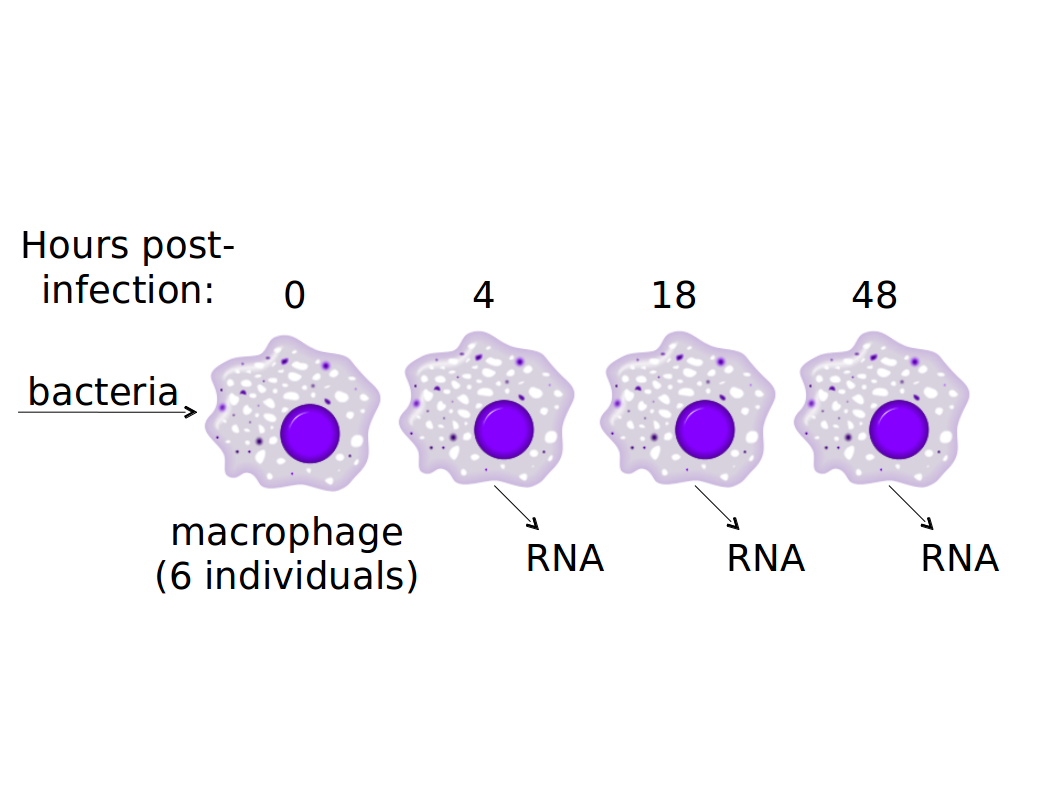
\includegraphics[width=5in]{img/ch02/fig-S01-study-design.png}
\caption[Study design.]{\textbf{Study design.} We infected
  monocyte-derived macrophages isolated from six healthy donors with
  the bacteria described in Table \ref{tab:bacteria}. We isolated RNA
  for sequencing at 4, 18, and 48 hours post-infection.}
\label{fig:ch02-study-design}
\end{figure}


